\subsection{Software:}\label{sc:software}
The application has been written as mentioned previously with the augmented reality technology in mind.
Due to this the application has been built with object-oriented approach.
This can be seen in how the objects are created.
To start with there is a base game object which has variables and functions that are required by all objects in the application.

This class is then inherited from for the marker object which is designed around being relative to an augmented reality marker.
This object has functions needed to do this such as setting an augmented reality matrix and building the world matrix based upon this new matrix.
This is the type of the objects used to cover the augmented reality markers in the game.

The cube object and the puzzle objects do not inherit from these class but they do instantiate other classes.
The cube object class instantiate both the puzzle object and the marker object classes.
While the puzzle object class instantiates a game object.
All this can be seen in Figure \ref{fig:ClassDiagrams} with the blue arrows representing inheritance and red arrow representing instantiation.
Another class that inherits is the augmented reality camera class as it adds functionality to the camera class that is specific to augmented reality applications.

\begin{figure}[ht!]
	\label{fig:ClassDiagrams}
	\centering
	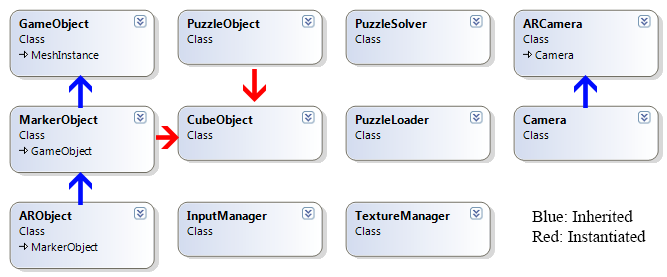
\includegraphics[width=\textwidth]{images/ClassDiagram2.PNG}
	\caption{Class Diagram}
\end{figure}

As well as using object-oriented approach to the objects used in the application is a Singleton pattern which is used for a number of the classes that manage particular objects or only need to be created once.
Currently in Figure \ref{fig:ClassDiagrams} the class that use the singleton pattern are Texture Manager, Input Manager, and the Puzzle Loader and Solver classes.
These classes use the pseudo code shown in Figure \ref{sc:singleton_pattern} to create only one instance of itself in addition with the constructor being a private function.
This code is based upon an example provided by \cite{codeproject2002}. 
As mentioned previously the reason for using this pattern is it allows for the classes to be created once it also allows for the class to be used in different objects whilst being only initialised once, which is very useful for the Texture Manager.

\begin{figure}[h|]
\centering
\begin{lstlisting}
ObjectType* GetObject(){
	if no instance of ObjectType{
		Create new ObjectType;
		set instance flag;
	}else{
		return already created ObjectType;
	}
}
\end{lstlisting}
\caption{Singleton Pseudo Code}
\label{sc:singleton_pattern}
\end{figure}

Figure \ref{sc:puzzle solver} shows pseudo code for the process used to check that the user has solved the puzzle.
The application checks by following the path generated by the tiles. For the first run the location of the tile is the location of the start tile.
The algorithm checks to see if the current tile is an end tile, which will be removed from the end tile list if it is.
If there are no more end tiles then the puzzle has been completed and the loop is exited.
Next each direction is check to see if it can move in that direction without leaving the bounds of the puzzle or entering a tile which isn't connected.
If it finds a direction store it and check the other directions.
If another direction has been found then add the tile to a list to be jumped back to later if the path hits a dead end. Once all directions have been check move to the next location and run again.
This process is repeated until all the ends are found or there are no more tiles to move to.

\begin{figure}[h!]
\centering
\begin{lstlisting}
Set current location to be that of the start tile
while(running){
	if(end tile){
		remove from the end list
	}
	if(end list empty){
		solved puzzle;
	}
	if(direction clear){
		if(no new direction){
			set new direction
		}else{
			add tile to list if haven't already been added
		}
	}
	move to the new tile based on direction found
	if(no new direction){
		check tile list
		if(empty){
			no solution and exit loop
		}else {
			jump to new tile
		}
	}
}
\end{lstlisting}
\caption{Puzzle Solver Pseudo Code}
\label{sc:puzzle solver}
\end{figure}

This process is run every time the user either presses the on screen solver button or the Select button.
The reason for waiting for user input rather than checking constantly or after every tile change is doing it that would take use a lot of resources that are not needed.
Also waiting for user input stops the user from accidental solving the puzzle.